\chapter{Einleitung}\label{einleitung}
\addthumb{Einleitung}{\huge{\textbf{\thechapter.}}}{white}{haw_rot} 

Ziel dieser Abschlussarbeit ist die Entwicklung einer Software zur medizinischen Bildverarbeitung. Eine modulare und flexible Architektur soll eine leichte Erweiterbarkeit sowohl für Entwickler (Erstellen eigener Werkzeuge) als auch den Anwender (Integration selbst implementierter Bildverarbeitungsalgorithmen) ermöglichen.\\
Das Programm soll für Forschung und Lehre im Labor für medizinische Bildverarbeitung, Algorithmen und Krankenhaus IT eingesetzt werden. Nach einer Vorstellung des Labors und dem zugehörigen Studiengang der biomedizinischen Technik erfolgt die Ermittlung der Anforderungen der Software. Aufbauend werden die Grundlagen medizinischer Daten- und Bildformate dargestellt. Der Fokus dieses Grundlagenkapitels liegt auf dem DICOM-Standard und den Eigenschaften der medizinischen Bilddaten. Die folgenden Kapitel erläutern die Softwarearchitektur sowie die Implementierung. Praktische Anwendungsbeispiele schließen die technischen Aspekte der Arbeit ab. Die folgende Diskussion zeigt Erweiterungsmöglichkeiten für die zukünftige Entwicklung auf.

\section{Der sechste Kondratieff-Zyklus}
Im Jahr 1926 veröffentlichte der Wirtschaftswissenschaftler Nikolai D. Kondratieff (* 1892, \dag 1938) die Theorie \glqq Die Langen Wellen der Konjunktur\grqq\ \cite{hensen:gesundeGesellschaft}.
Leo Nefiodow erweiterte 2006 die Theorie, damit die Entwicklung des 20. Jahrhunderts einfließen konnte.\\
Kondratieff zeigte, dass sich die gesellschaftliche Wandlung nicht willkürlich vollzog. Seit der Industrialisierung Mitte des 18. Jahrhunderts stand der Wohlstand der Gesellschaft in direkter Beziehung zu besonderen Erfindungen. Er betrachtete die Phasen des Wohlstandes und die direkt folgende Wirtschaftskrise und entdeckte die später nach ihm benannten \glqq Kondratieff-Zyklen\grqq\.
Wie in Abbildung \ref{zyklen} zu sehen ist, war die Dampfmaschine die erste Basisinnovation\footnote{Basisinnovationen müssen nach Nefiodow vier Eigenschaften erfüllen: Entstehung eines neuen Marktes mit vielen Arbeitsplätzen; Innovation bestimmt den Zyklus; Basisinnovationen haben einen Zyklus von 40 - 60 Jahren; Sie bestimmen die Entwicklungsrichtung} und revolutionierte die Textilindustrie.\cite{wieden:liquidwork}

%\begin{wrapfigure}{c}{10cm}
%\centering
%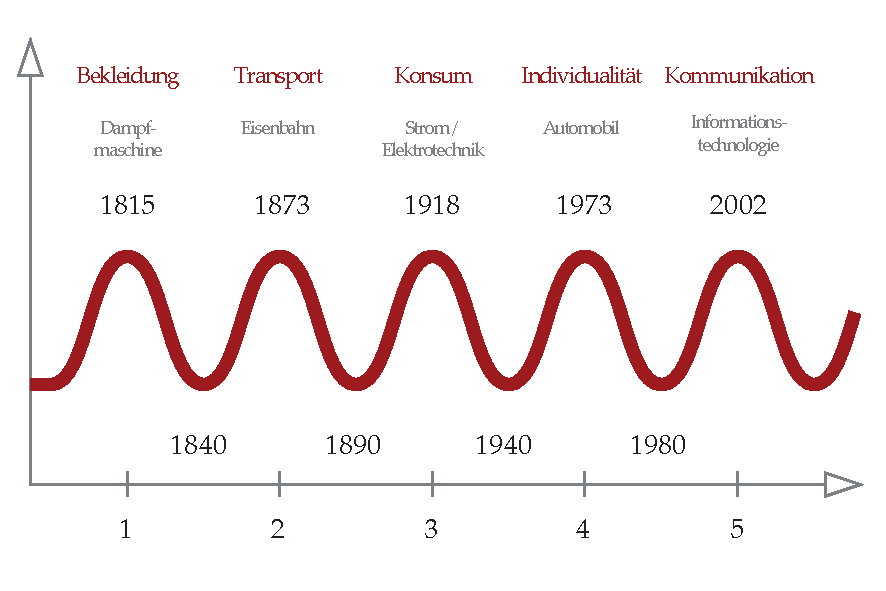
\includegraphics[width=8cm]{./img/zyklen.pdf}
%\caption{Kontratieff Zyklen}
%\label{zyklen}
%\end{wrapfigure}

\begin{figure}[htbp]
  \vspace{0.5cm}
  \centering
  \fbox{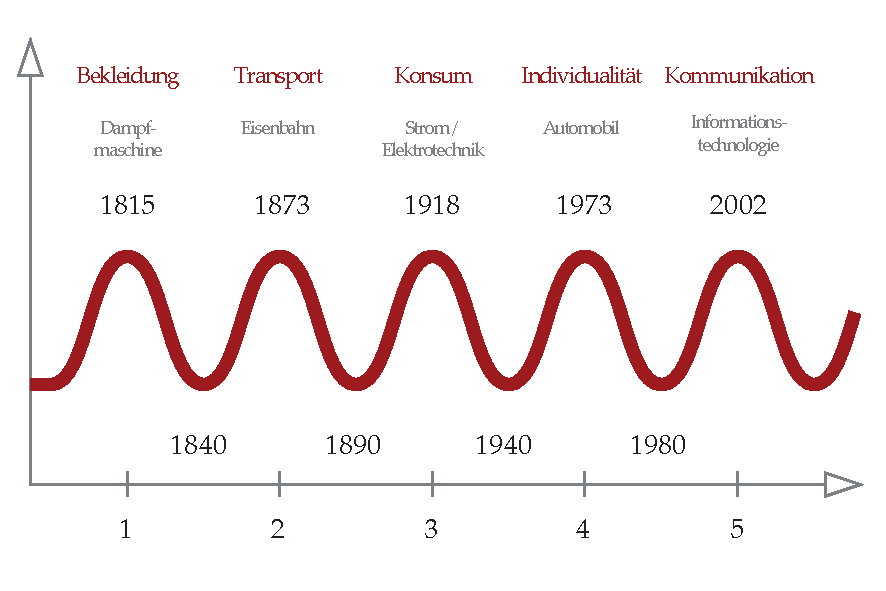
\includegraphics[angle=0,width=12cm]{./img/zyklen.pdf}}
  \caption{Kondratieff-Zyklen}
  \label{zyklen}
  \vspace{0.5cm}
\end{figure}

Diese Erfindung gilt als Beginn des ersten Kondratieff-Zyklus. Vor dem maschinellen Betrieb wurden Spinnräder noch manuell bedient und Kleidung war teuer. Die dampfbetriebenen Webstühle steigerten
die Effizienz um das 200-fache. In den 20er Jahren stagnierte die Branche, da die Rohstoffbeschaffung und Warenverteilung das Maximum der Effizienz erreicht hatte. Mit der Erfindung der Eisenbahn gelang der Übergang vom ersten in den zweiten Zyklus. In den folgenden Jahren konnte nun das Bedürfnis nach verbesserten Transportmöglichkeiten gestillt werden.\\
Dampfmaschine, Eisenbahn, Strom, Motor und der Mikrochip stehen alle für eine Basisinnovation, die zukünftige Gesellschaften geprägt haben. Im lauf der Zeit verschwinden die Erfindungen aus dem Bewusstsein der Menschen und werden zu Gegenständen des Alltags. Motor und Mikrochip sind so stark im gesellschaftlichen Leben verankert, dass sie nicht mehr direkt wahrgenommen werden. Betrachtet man eine elektrische Zahnbürste, ist es selbstverständlich, dass die Energie aus dem Stromnetz bezogen und der Bürstenkopf von einem Motor angetrieben wird.\\
Das Jahr 2002 gilt als Höhepunkt des fünften Kondratieff-Zyklus und die Gesellschaft befindet sich gerade im Übergang zum Sechsten. Noch fehlt die aktuelle Basisinnovation und auch das zu nächste stillende Bedürfnis ist nach Individualität und Kommunikation(Abbildung \ref{zyklen}) noch nicht bestimmt.\\
Nach Nefiodow \cite{nefiodow:gesundheit} gibt es vier Möglichkeiten welcher Markt in Zukunft den sechsten Kondratieff prägen wird:
\begin{itemize}
  \item \textbf{Informationsmarkt} \\
  		Mobile Geräte und Soziale Netzwerke sind maßgebend für diesen Markt. So verhalf der Kurznachrichtendienst Twitter zum sogenannten \glqq Arabischen Frühling\grqq\, durch die blitzschnelle Kommunikation über das Netz\footnote{http://www.heise.de/tr/blog/artikel/Wie-funktioniert-die-Twitter-Revolution-1761481.html \\aufgerufen am 06.01.2014}.
  \item \textbf{Bio - und Nanotechnologie} \\
  		Die Erfindung des Mikroskops und die Entschlüsselung der DNA im Jahr 2000 gilt als Basisinnovation. Anfangs wurden die Erkenntnisse nur in Medizin und Pharmazie angewendet. Heute profitiert auch die Landwirtschaft und Lebensmittelindustrie davon.
  \item \textbf{Umwelttechnologie}
  		Auch der Bereich Umwelttechnologie sorgte für einen Zuwachs an Arbeitsplätzen in Deutschland und Österreich. Zusätzlich siedelten sich Unternehmen besonders in ländlichen und strukturschwachen Gebieten an. \cite[S. 107]{nefiodow:gesundheit}.
  \item \textbf{Gesundheit}
  		Der Gesundheitsmarkt vereint technologische Komponenten wie die Medizintechnik und psychosoziale Gesundheit. Es erfolgt ein Wechsel vom heutigen \glqq Krankheitswesen\grqq\ zum Gesundheitswesen, angefangen von der Burnout-Prophylaxe, Gesundheitstourismus zur Bionik und künstlichen computergesteuerten Prothesen.
\end{itemize}

\section{Wachstumsmarkt Gesundheit}

Nach Granig\cite{nefiodow:gesundheit} ist der Gesundheitsbereich der derzeit am schnellsten wachsende Markt\footnote{Gemessen am Anteil der Branche am Bruttoinlandsprodukt}. Die Bevölkerung ist gewillt in die eigene Gesundheit zu investieren und die Unternehmen positionieren sich im Gesundheitsbereich (Siemens beispielweise verstärkt sich im Bereich der Medizintechnik \cite[S.111, 112]{nefiodow:gesundheit})
Die Bio- und Nanotechnologie und die Medizintechnik ähneln sich in einigen Bereichen. Sowohl Siemon Cord \cite{cord:innovation} als auch Granig \cite[Seite 116 f]{nefiodow:gesundheit} sprechen davon, dass der Markt sich nur gehemmt entwickeln kann. Grund dafür sind sowohl für die Nano- als auch Medizintechnik veraltete Vorschriften und auch ethische Hürden, die es zu überwinden gilt. Granig nennt hierzu unter anderem die Mensch-Computer-Einheit \cite[S.117]{nefiodow:gesundheit}(computergesteuerte Prothesen und künstliche Ersatzteile).\\
Die Entwicklung für den wachsenden Markt finden in den Unternehmen statt. Der Grundstein für Innovation wird jedoch bei den Studierenden der Hochschulen und Universitäten gelegt. Die Bildungseinrichtungen werden ein zentrales Standbein für den kommenden sechsten Kondratieff mit einem Schwerpunkt Bio-, Medizintechnik und Gesundheit sein.

%Cord schreibt, dass 100\% des Wissens der Biotechnik aus Hochschulwissen stammt (allerdings aufgrund der erwähnten Einschränkungen noch nicht ökonomisch verwertet werden kann). Zwar trifft diese %hohe Prozentzahl nicht auf die Medizintechnik zu, da viel Entwicklung in den Unternehmen stattfindet, doch der Grundstein für Innovation wird bei den Studierenden der Hochschulen und %Universitäten gelegt. Die Bildungseinrichtungen werden ein zentrales Standbein für den kommenden sechsten Kondratieff mit einem Schwerpunkt Bio-, Medizintechnik und Gesundheit sein.

\section{Der Studiengang Biomedizinische Technik}\label{einleitung:biomedTechnik}
In einem Onlineartikel vom Februar 2012\footnote{https://www.haw-landshut.de/aktuelles/news/news-archiv/news-detailansicht/article/neuer-studiengang-biomedizinische-technik-vielfaeltige-berufschancen.html \\ abgerufen am 10.01.2014} veröffentlichte die Hochschule Landshut, dass ab dem Wintersemester 2012 der neue Bachelorstudiengang \glqq Biomedizinische Technik\grqq\ angeboten wird. Auch der Artikel beschreibt, ähnlich wie Granig, die Medizintechnik als Wachstumsmarkt und bestätigt, auch durch die Einführung des Studiengangs, das gesellschaftlich gesteigerte Interesse am Gesundheitswesen.\\
Während des Studienverlaufs \cite{hsla:modulBMT} erwerben die Studierenden vor allem im zweiten Studienabschnitt Kenntnisse im Bereich der Medizintechnik. Die Ausbildung behandelt unter Anderem bildgebenden Systeme, medizinische Bildverarbeitung und minimalinvasive Therapieverfahren.\\
Für die Ausbildung stehen Labore mit den benötigten Geräten zur Verfügung, um mit dem theoretischen Wissen praktisch zu experimentieren.

\section{Das Labor für medizinische Bildverarbeitung, Algorithmen und Krankenhaus IT}\label{einleitung:labor}
Das Labor erfüllt zwei Aspekte. Die Ausstattung steht für Forschungs- und Entwicklungsarbeiten zur Verfügung. Gemeinsame Forschungsprojekte von Hochschule und Krankenhäusern oder Unternehmen können hier umgesetzt werden.
Für die Lehre soll Studierenden die Möglichkeit geboten werden, den Prozess der medizinischen Bildverarbeitung anschaulich und praxisnah zu erleben. Mittels Doppler-Ultraschallgerät können Bilddaten erzeugt und anschließend an das Picture Archiving and Communication System\footnote{Ein PACS dient als zentraler Bildspeicher, der über das Netzwerk angesprochen werden kann. Medizinische Geräte legen dort die Bilddaten ab, während die Software zu Betrachtung die Daten vom PACS holt} (PACS) gesendet werden. Anschließend können Algorithmen zur Bildvorverarbeitung, Merkmalsextraktion oder auch Segmentierung implementiert und getestet werden.\\
Medizinische Bildformate unterscheiden sich maßgeblich von allgemein bekannten Formaten wie JPEG oder Bitmaps, daher sind zur Betrachtung sogenannte DICOM-Viewer\footnote{DICOM (Digital Imaging and Communications in Medicine) ist der heutige Standard der medizinischen Informationsverarbeitung und wird in den folgenden Kapiteln näher erläutert. Die Viewer ermöglichen die Betrachtung der Bilddaten} notwendig. So enthalten medizinische Formate neben den reinen Bilddaten noch viele weitere Informationen, zum Beispiel Patientendetails oder die tatsächliche Lage des Patienten in der realen Welt zum Zeitpunkt der Aufnahme.
Mit Hilfe der DICOM-Viewer lassen sich die erzeugten Bilder betrachten und grundlegende Operationen auf diesen anwenden (dazu zählt beispielsweise die Skalierung oder Verschiebung des Bildes). Komplexe Bildverarbeitungsalgorithmen können allerdings nicht ausgeführt oder selbst implementiert werden.\\
Für Forschung und Lehre wird eine Software benötigt, die sowohl die Grundfunktionen der Betrachtung liefert, als auch eine Schnittstelle zur eigenen Erweiterung zu Verfügung stellt.

